\documentclass{beamer}

\usepackage{graphicx,hyperref,url}

\usepackage[T1]{fontenc}    %%% UNICODES etc
\usepackage[utf8]{inputenc}

\usepackage{booktabs}
\usepackage[brazil]{babel}
\usepackage{lmodern, comment}
\usepackage{amsmath,amssymb,amstext}
\usepackage{xcolor}
\usepackage{pifont}
%%%\usepackage{fontspec}
\usepackage{marvosym}

%%% TO DISCOVER ERRORS 
%\DeclareUnicodeCharacter{00B4}{\ensuremath{\theta}}

%% FOR ASP
\usepackage{listings}
\lstset{basicstyle=\ttfamily,escapechar=\%,escapeinside={\#(}{\#)}}


%%% FIGS \graphicspath{{figures/}{../figures/}{C:/Users/me/Documents/project/figures/}}

\graphicspath{ {figures/} {../ia_combinatoria/figures/} }
%%%%\graphicspath{ {/home/user} }
\definecolor{azulclaro}{rgb}{0.9,0.9,0.9}
\definecolor{mygreen}{rgb}{0,0.6,0}
\definecolor{mygray}{rgb}{0.5,0.5,0.5}
\definecolor{mymauve}{rgb}{0.58,0,0.82}
\definecolor{darkgray}{rgb}{.4,.4,.4}
\definecolor{purple}{rgb}{0.65, 0.12, 0.82}


\lstset{ 
  %  label={pgm_ex01},
    backgroundcolor=\color{azulclaro}, 
    language=Haskell, %%Miranda,%%Perl,%%%Python, %%Mercury,
    showstringspaces=false,
    basicstyle=\bf\scriptsize\ttfamily,
%%      basicstyle= \footnotesize %%% TESTAR
%%      keywordstyle=\bfseries\color{green!40!black},
    keywordstyle=\textbf{\color{mygreen}}, 
    otherkeywords={*, \%, array, constraint, solve, output,  show, "/\", satisfy, set, of, if, then, elseif, float, search},
%%  keywordstyle=\color{blue},       % keyword style
%%    commentstyle=\itshape\color{purple!40!black},
      commentstyle=\color{orange},    % comment style
      identifierstyle=\color{blue},
      stringstyle=\color{orange},
      stringstyle=\color{mymauve},
      numbers=left,  % where to put the line-numbers; possible values are (none, left, right)
      numbersep=5pt,   % how far the line-numbers are from the code
      numberstyle=\tiny\color{magenta},
      keepspaces=true      
    % %caption={LEGENDA no source PASCAL ficou OK},
}



\title[Combinatorial  Optimization] % (optional, use only with long paper titlebg=blue!20!white,s)
{Tug of War Problem with \\ \textit{Answer Set Programming -- clingo}\\ An Encoding}
%\subtitle
%{About some things}
\author[Claudio Cesar de Sá] % (optional, use only with lots of authors)
{Claudio Cesar de Sá}%\inst{1}
% - Give the names in the same order as the appear in the paper.
% - Use the \inst{?} command only if the authors have different
%   affiliation.

\institute[WhatsTV]{Independent Researcher}

% - Use the \inst command only if there are several affiliations.
% - Keep it simple, no one is interested in your street address.

\date[\today] % (optional, should be abbreviation of conference name)


\begin{document}

\begin{frame}
  \titlepage
  
\end{frame}



% Structuring a talk is a difficult task and the following structure
% may not be suitable. Here are some rules that apply for this
% solution: 

% - Exactly two or three sections (other than the summary).
% - At *most* three subsections per section.
% - Talk about 30s to 2min per frame. So there should be between about
%   15 and 30 frames, all told.

% - A conference audience is likely to know very little of what you
%   are going to talk about. So *simplify*!
% - In a 20min talk, getting the main ideas across is hard
%   enough. Leave out details, even if it means being less precise than
%   you think necessary.
% - If you omit details that are vital to the proof/implementation,
%   just say so once. Everybody will be happy with that.

%%%%%%%%%%%%%%%%%%%%%%%%%%%%%%%%%%%%%%%%%%%%%%%%%%%%%%%


\begin{frame}

\begin{block}{Road map of this presentation:}
%  \tableofcontents

\begin{enumerate}

  \item  About the  ASP (clingo) -- previous presentation (done)
  \item  Requisites -- previous presentation (done)
  \item  Tug of War (well knowed problem from competitive programming sites and contests)
  \item  A modelling in ASP
  \item  A solution in clingo
  \item  Using Python's code inside of ASP
  \item  Conclusions

  \end{enumerate}

\end{block}

\pause
\textbf{\textcolor{red}{Attention: some background in logic and declarative language is recommended!}}


\end{frame}


%%%%%%%%%%%%%%%%%%%%%%%%%%%%%%%%%%%%%%%%%%%%%%%%%%%%%%%
\begin{comment}
\section{Para efeitos de TEMPLATE}
\begin{frame}
\frametitle{Nome do SLIDE}
\begin{block}{Nome do Bloco}
  \begin{itemize}
   \item T1

    \item<2-> T2

    \item<3-> T3

  \item<4-> 

    \item<5-> 
    
        \item<6-> 
    \end{itemize}
  
\end{block}

\end{frame}
\end{comment}
%%%%%%%%%%%%%%%%%%%%%%%%%%%%%%%%%%%%%%%%%%%%%%%%%%%%%%%




%%%%%%%%%%%%%%%%%%%%%%%%%%%%%%%%%%%%%%%%%%%%%%%%%%%%%%%%%
%%%%%%%%%%%%%%%%%%%%%%%%%%%%%%%%%%%%%%%%%%%%%%%%%%%%%%\

\section{Definitions -- Graph coloring:}
\begin{frame}[fragile] 
	%\frametitle{Graph coloring -- a set of problems related}
	\frametitle{Tug of War Problem}
		
	
\begin{figure}[tbp]
  \centering
%	 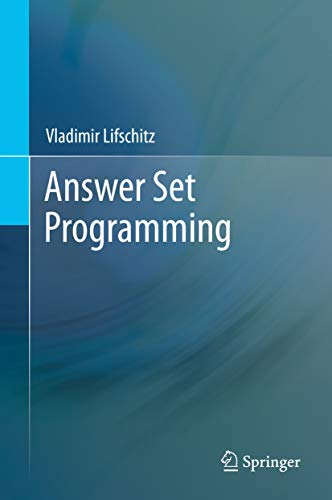
\includegraphics[width=0.4\textwidth , height=0.55\textheight]{cover_book_vladmir.jpg}
	 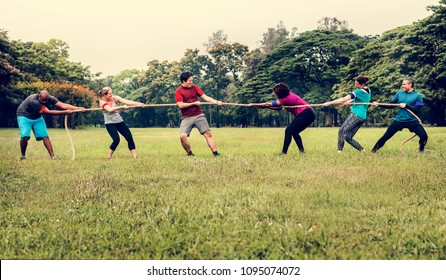
\includegraphics[width=0.9\textwidth , height=0.7\textheight] {fig01-tug-war.jpg}
  \caption{Practical application of this problem}
	
	\end{figure}

\end{frame}

\begin{frame}[fragile] 

	\frametitle{Tug of War} 

From: \textcolor{blue}{\url{https://www.geeksforgeeks.org/tug-of-war/}}\\
and/or \textcolor{blue}{\url{https://www.codechef.com/problems/CO319TSH}}

\begin{block}{}

Given a set of $n$ integers, divide the set in two subsets of $n/2$ sizes each such that the difference of the sum of two subsets is as minimum as possible. If $n$ is even, then sizes of two subsets must be strictly $n/2$ and if $n$ is odd, then size of one subset must be $(n-1)/2$ and size of other subset must be $(n+1)/2$.
\end{block}

\end{frame}

%%%%%%%%%%%%%%%%%%%%%%%%%%%%%%%%%%%%%%%%%%%%%%%%%%%%%%%%%%%%%%%%%%%%%

\begin{frame}[fragile] 

	\frametitle{Examples} 

From: \textcolor{blue}{\url{https://www.geeksforgeeks.org/tug-of-war/}}

\begin{block}{}
  \begin{itemize}
  \setlength\itemsep{7pt}

  \item Example 1: let given set be \{3, 4, 5, -3, 100, 1, 89, 54, 23, 20\}, the size of set is $10$. Output for this set should be \{4, 100, 1, 23, 20\} and \{3, 5, -3, 89, 54\}. Both output subsets are of size 5 and sum of elements in both subsets is same (148 and 148). 

  \item Let us consider another example where $n$ is odd. Let given set be \{23, 45, -34, 12, 0, 98, -99, 4, 189, -1, 4\}. The output subsets should be \{45, -34, 12, 98, -1\} and \{23, 0, -99, 4, 189, 4\}. The sums of elements in two subsets are 120 and 121 respectively.


\item This problem is beauty: \emph{easy to understand, hard to solve it}!

  \end{itemize}
 \end{block}

\end{frame}


\begin{frame}[fragile] 

	\frametitle{Comments} 

\begin{block}{}
  \begin{itemize}
 % \setlength\itemsep{4pt}
 \item Again: all the combinations must be found!
  \item Input: a set of numbers, in our implementation an array, aiming a possible repetitions of these numbers.
  
  \item Output: two sets with the same size/cardinality, or with difference of one number for set A or B. 
  
  \item Complexity:	NP-Complete (all the combinations must be examined) -- Set partition problem is NP complete -- \url{https://www.geeksforgeeks.org/set-partition-is-np-complete/}
  
  \item Optimization: NP-Hard, due the minimum value of the absolute difference between the sum of two  sets.
  \end{itemize}
 \end{block}

\end{frame}

%%%%%%%%%%%%%%%%%%%%%%%%%%%%%%%%%%%%%%%%%%%%%%%%%%%%%%%%%%%%%%%%%%%%%

%%%%%%%%%%%%%%%%%%%%%%%%%%%%%%%%%%%%%%%%%%%%%%%%%%%%%%%
\section{Modelling}
\begin{frame}[fragile] 
	\frametitle{Some comments and motivation:}
	
\begin{block}{}
  \begin{itemize}
  % \setlength\itemsep{4pt}

 \item I solved it in Minizinc!

  \item Some approaches for this problem can be taken: Simulated Annealing, Ant Colony, Depth-First Search,  meta-heuristics, ... etc.

\item Dynamic Programming (DP) is the most suitable for contest programming

  \item The full code discussed here is found in:\\ {\bf \textcolor{blue}{\url{https://github.com/claudiosa/CCS/tree/master/asp_Answer_Set_Programming/tug_of_war.lp}}}

  \item I will be commenting the modelling in parts 

   \end{itemize}
 \end{block}
	
	
%\textcolor{red}{xxxxxxxxxxxxxxxxxxxxxxxxxxx!}	
\end{frame}
%%%%%%%%%%%%%%%%%%%%%%%%%%%%%%%%%%%%%%%%%%%%%%%%%%%%%%%
\begin{frame}[fragile] 
\frametitle{Modelling: }

\begin{itemize}
  \item The input values of this problem (an array and its size)
  \pause
  \item A help from Python here, it is discussed at the end this modelling

 \end{itemize}

	
{\small
\begin{verbatim}
$ cat inp_2_tug_of_war.txt
#const n=11.
weights(1,23).  weights(2,45).  weights(3,-34). weights(4,12). 
weights(5,0).   weights(6,98).  weights(7,-99). weights(8,4). 
weights(9,189). weights(10,-1). weights(11,4).
\end{verbatim}
}	

\begin{itemize}
\item Reminding our second case -- example:\\
{\bf \{23, 45, -34, 12, 0, 98, -99, 4, 189, -1, 4\}}

\item {\bf \textcolor{red}{Already converted in ground terms}}

\end{itemize}

\textcolor{red}{\rule{\textwidth}{1.7pt} } 

\end{frame}


%%%%%%%%%%%%%%%%%%%%%%%%%%%%%%%%%%%%%%%%%%%%%%%%%%%%%%%

\begin{frame}[fragile] 
	\frametitle{Creating the possible sets as solutions:}
	

	
{\small
\begin{verbatim}
% creating sets 01 and 02
 { set_01(I,W) }  :-  weights(I,W).
 { set_02(I,W) }  :-  weights(I,W).

%%% a CONSTRAINT here: these sets are disjunctives
:- set_01(I,_), I = 1..n, set_02(J,_), J = 1..n, I == J.
%% any set has the same element referenced by an index

\end{verbatim}
}	
\textcolor{red}{The $n$ value was defined previously!}\\
\textcolor{red}{Here is the trick of this modelling -- think about it!}\\
\textcolor{red}{\rule{\textwidth}{1.7pt} } 
\end{frame}


%%%%%%%%%%%%%%%%%%%%%%%%%%%%%%%%%%%%%%%%%%%%%%%%%%%%%%%
\begin{frame}[fragile] 
	\frametitle{Counting and summing the elements of each set:}
	
	Extensive use of \textcolor{blue}{{\bf aggregate functions}}: {\bf \texttt{\#count}} and {\bf \texttt{\#sum}}
	
{\small
\begin{verbatim}
%% counting elements of sets 01 and 02 by index
n_1(N) :- N = #count{I: set_01(I,W) }.
n_2(N) :- N = #count{I: set_02(I,W) }.
size(N) :- N = #count{I: weights(I,W)}.

%% summing all elements of sets 01 and 02
sum_set_01(X) :- X = #sum{W,I : I= 1..n, set_01(I,W)}.
sum_set_02(X) :- X = #sum{W,I : I= 1..n, set_02(I,W)}.
\end{verbatim}
}	
%\textcolor{red}{Basically, that's all!}
\textcolor{red}{\rule{\textwidth}{1.7pt} } 
\end{frame}



\begin{frame}[fragile]
	\frametitle{About the size of each set:}

Reminding:
{\small
\begin{verbatim}
n_1(X): X is the cardinality of set_1 
n_2(Y): Y is the cardinality of set_2 
size(N): N is the cardinality of original set
...
so
..
% constraint 2 ... set 1 and 2 .. are almost the same size
:- n_1(X), n_2(Y) , X - Y > 1 .  % not allowed  IF |X|  > |Y|  
:- n_1(X), n_2(Y) , Y - X > 1.   % not allowed  IF |Y|  > |X|
% constraint 1 ... sum of size sets are the same
:- n_1(X), n_2(Y) , size(N) , (X+Y) != N.

\end{verbatim}
}	
\textcolor{red}{Securely, this part can be improved !}\\
\textcolor{red}{\rule{\textwidth}{1.7pt} } 
\end{frame}


%%%%%%%%%%%%%%%%%%%%%%%%%%%%%%%%%%%%%%%%%%%%%%%%%%%%%%%%%%%%%%%%%%%%%%%%%%%%%%%%%%%%%%%%%%%%%%


\begin{frame}[fragile]
	\frametitle{Preparing for the optimization:}


{\small
\begin{verbatim}
%% the abs works fine
diff(Z) :- sum_set_01(X), sum_set_02(Y),  Z = |Y - X|. 
%% #abs(Y-X).

%% if "a perfect" balance  -- no differences of weight
answer('y_YES') :- diff(0).
answer('n_NO') :- diff(Z), Z != 0.

%% A minimizations on this difference
#minimize{ Z : diff(Z) }.

\end{verbatim}
}	
\textcolor{red}{\rule{\textwidth}{1.7pt} } 
\end{frame}
%%%%%%%%%%%%%%%%%%%%%%%%%%%%%%%%%%%%%%%%%%%%%%%%%%%%%%%
\begin{frame}[fragile]
	\frametitle{The outputs:}

{\small
\begin{verbatim}
#show n_1/1. 
#show n_2/1.
%#show size/1.

%% sets obtained
#show set_01/2. 
#show set_02/2.
%% sum of each side 
#show sum_set_01/1.
#show sum_set_02/1.
#show diff/1.
#show answer/1.
\end{verbatim}
}	
\textcolor{red}{\rule{\textwidth}{1.7pt} } 
\end{frame}




%%%%%%%%%%%%%%%%%%%%%%%%%%%%%%%%%%%%%%%%%%%%%%%%%%%%%%%
%\begin{frame}[allowframebreaks]
\begin{frame} [fragile]
\frametitle{An output:}
	
{\small
\begin{verbatim}
$ clingo tug_of_war.lp inp_2_tug_of_war.txt 
qclingo version 5.3.0
Reading from tug_of_war.lp ...
Solving...
Answer: 1
set_02(4,12) set_02(5,0) set_02(3,-34) set_02(7,-99) 
set_02(10,-1) 
set_01(1,23) set_01(2,45) set_01(6,98) set_01(8,4) 
set_01(9,189) set_01(11,4) 
sum_set_02(-122) sum_set_01(363) diff(485) 
answer('n_NO') n_2(5) n_1(6)
Optimization: 485
Answer: 2
...........................................
\end{verbatim}
\textcolor{red}{Many lines omitted!}\\
\textcolor{red}{\rule{\textwidth}{1.7pt} } 
}	
\end{frame}

\begin{frame} [fragile]
\frametitle{An output:}
\textcolor{red}{Finally in the answer 12:}
{\small
\begin{verbatim}
...
Answer: 12    
set_02(2,45) set_02(4,12) set_02(6,98) set_02(3,-34) 
set_02(10,-1) 
set_01(1,23) set_01(5,0) set_01(8,4) set_01(9,189) 
set_01(11,4) set_01(7,-99) 
sum_set_02(120) sum_set_01(121) diff(1) 
answer('n_NO') n_2(5) n_1(6)
Optimization: 1
OPTIMUM FOUND

Models       : 12
  Optimum    : yes
Optimization : 1
Calls        : 1
Time         : 1.181s (Solving: 0.58s 1st Model: 0.03s Unsat: 0.06s)
CPU Time     : 1.181s

\end{verbatim}
}	
\end{frame}

\begin{frame} [fragile]
\frametitle{Using Python's code inside of ASP}

\begin{itemize}
\item A big help from Adam Smith (Postasco mailing list)
\item How to deal with input and output values in ASP?
\pause
\item Some snippets of code in Python!
\item The code discussed here:\\
\textbf{\textcolor{blue}{\url{convert_input_value_in_terms_Python.lp}}}

\end{itemize}
	
\end{frame}

\begin{frame} [fragile]
\frametitle{An example:}
	
{\small
\begin{verbatim}
#script (python)
def my_size(*terms):
    i=0
    for term in enumerate(terms):
       i+=1
    return i
#end.

#script (python)
def multiset( *terms ):
  result = []
  for i , term in enumerate(terms):
    """ List of Pairs """
    result.append( (i+1, term) )
  return result
#end.
...
\end{verbatim}
}	
\end{frame}

%%%%%%%%%%%%%%%%%%%%%%%%%%%%%%%%%%%%%%%%%%%%%%%%%%%%%%%%%%%%%%%%%%%%%%%%%%%%%%%%%%%%%%%%%%%%%%%%%%%%%%%%%%%%%%
\begin{frame} [fragile]
\frametitle{Using Python's functions embedded in ASP:}
	
{\small
\begin{verbatim}
...
weights(I,W) :- (I,W) = @multiset( 23, 45, -34, 12, 0  ).
size(S) :- S = @my_size(1,2,3,4,9999999999).
...
\end{verbatim}
}
\textcolor{red}{\rule{\textwidth}{1.7pt} } 

{\small
\begin{verbatim}
$ clingo convert_input_value_in_terms_Python.lp
...
Answer: 1
size(5) weights(1,23) weights(2,45) weights(3,-34) 
weights(4,12) weights(5,0)
SATISFIABLE
Models       : 1
...
\end{verbatim}
}	
\textcolor{red}{\rule{\textwidth}{1.7pt} } 
\end{frame}

%%%%%%%%%%%%%%%%%%%%%%%%%%%%%%%%%%%%%%%%%%%%%%%%%%%%%%%%%%%%%%%%%%%%%%%%%%%%%%%%%%%%%%%%%%%%%%%%%%%%%%%%%%%%%%

\begin{frame}[fragile] 
	\frametitle{Conclusions:}
	
\begin{block}{}
\begin{itemize}

  \item ASP is strongly declarative (roots from the logic to attack the  representation and combinatorial problems)
  
  \item A methodology generate and test to developing
    
  \item ASP's workflow, modeling, grounding, solving
    (and optimizing)
    %\smallskip
  \item Here, we solved \emph{the tug of war problem}. Easy to understand, but is is a combinatorial problem.
  
  \item Allows you to embbed a Python coding in order to minimize the difficulties (\Smiley) of input and output data
		
   \item An encoding in ASP is excellent exercise to keep your mind very active!

	\item Finally, a huge gratitude for the \textcolor{green}{\textbf{potassco-users list}}, always reactive for my silly doubts,  where I had been learning much.
		
	\end{itemize}
\end{block}
\end{frame}


%%%%%%%%%%%%%%%%%%%%%%%%%%%%%%%%%%%%%%%%%%%%%%%%%%%%
\section*{Contact}

\begin{frame}
\frametitle{Contact and comments (are must welcome\ \Smiley):}
  
\begin{block}{}
  % Keep the summary *very short*.
  \begin{itemize}
  \item \url{https://claudiocesar.wordpress.com/}
%   \item \url{https://github.com/claudiosa}
   \item \textcolor{red}{This presentation and the code discussed}:\\
   \textbf{\textcolor{blue}{\url{https://github.com/claudiosa/CCS/tree/master/asp_Answer_Set_Programming}}}
   \item There is a directory to Youtube!
   \item  The full code discussed here is found in:\\ \textbf{\textcolor{blue}{\url{https://github.com/claudiosa/CCS/tree/master/asp_Answer_Set_Programming/tug_of_war.lp}}}
    
   %\item In this  git, repository CCS $\Rightarrow$ asp...
   %%\item Email: \url{claudio.sa@udesc.br}
  \item \Letter: \url{ccs1664@gmail.com}
  \item This material has a partial support from WhatsTV Inc. \url{https://en.whatstv.com.br/}, here our gratitude!
  \item \textit{Thank you so much}!

  \end{itemize}
  \end{block}

\end{frame}


%%%%%%%%%%%%%%%%%%%%%%%%%%%%%%%%%%%%%%%%%%%%%%%%%%%%%%%
\end{document}
